\documentclass[a4paper]{article}

\def\nbook {Differential Equations and Linear Algebra}
\def\nbookshort {DeqLA}

\input{../headerdeqla}
\hfuzz=50pt

\begin{document}
\maketitle

\newpage
\tableofcontents

\newpage
\section{\textsf{8 - Fourier and Laplace Transforms}}

\subsection{\textsf{8.1 - Fourier Series}}
% QUESTION 1
\qs{8.1.1}{
\begin{enumerate}[label=(\alph*)]
	\item To prove that \( \cos\!\left(nx\right) \) is orthogonal to \( \cos\!\left(kx\right)  \) when \( k \neq n \), use the formula \( \!\left( \cos\!\left(nx\right) \right) \!\left( \cos\!\left(kx\right) \right) = \frac{1}{2} \cos\!\left(\!\left( n + k \right) x \right) + \frac{1}{2}\cos\!\left(\!\left( n - k \right) x \right) \). Integrate from \( x = 0 \) to \( x = \pi \). What is \( \int \cos^{2}\!\left(kx\right) \, dx \) ?
	\item From 0 to \( \pi \), \( \cos\!\left(x\right)  \) is \textbf{not} orthogonal to \( \sin\!\left(x\right)  \). The period has to be \( 2 \pi \):
	
		Find \( \displaystyle{\int^{\pi}_{0} \sin\!\left(x\right) \cos\!\left(x\right) \, dx } \) and \( \displaystyle{\int^{\pi}_{-\pi} \sin\!\left(x\right) \cos\!\left(x\right) \, dx} \) and 

		\( \displaystyle{\int^{2 \pi}_{0} \sin\!\left(x\right) \cos\!\left(x\right) \, dx } \).
\end{enumerate}}

\begin{enumerate}[label=(\alph*)]
	\item For \( k \neq n \), integrate
	\begin{align*}
		\int^{\pi}_{0} \cos\!\left(nx\right) \cos\!\left(kx\right)  \, dx & = \int^{\pi}_{0} \!\left[ \frac{1}{2} \cos\!\left(\!\left( n + k \right) x \right) + \frac{1}{2} \cos\!\left(\!\left( n - k \right) x \right) \right] \, dx & \\ 
										  & = \frac{1}{2} \!\left[ \frac{1}{n + k} \sin\!\left(\!\left( n + k \right) x \right) + \frac{1}{n - k} \sin\!\left(\!\left( n - k \right) x \right) \right] \Big|^{\pi}_{0} \\
										  & = 0
	\end{align*}
	When equality holds, we have
	\[
		\int^{\pi}_{0} \cos^{2}\!\left(kx\right) \, dx = \int^{\pi}_{0} \!\left[ \frac{1}{2} \cos\!\left(2kx\right) + \frac{1}{2} \right] \, dx = \frac{\pi}{2}
	\]
	\item I think the textbook has a typo. The integrand should be \( \sin\!\left(2x\right) \cos\!\left(x\right)  \).
	\begin{align*}
		\int^{\pi}_{0} \sin\!\left(2x\right) \cos\!\left(x\right) \, dx & = \int^{\pi}_{0} 2 \sin\!\left(x\right) \cos^{2}\!\left(x\right)  \, dx \\
										& =  -\frac{2}{3} \cos^{3}\!\left(x\right) \Big|^{\pi}_{0} \\
										& = \frac{4}{3}
	\end{align*}
	When we set the integral to the two other sets of bounds, we find
	\[
		-\frac{2}{3}\cos^{3}\!\left(x\right) \Big|^{\pi}_{-\pi} = -\frac{2}{3}\cos^{3}\!\left(x\right) \Big|^{2 \pi}_{0} = 0
	\]
\end{enumerate}

\newpage
% QUESTION 2
\qs{8.1.2}{Suppose \( F \!\left( x \right) = x \) for \( 0 \le x \le \pi \). Draw graphs for \( -2 \pi \le x \le 2 \pi \) to show three extensions of \( F \): a \( 2 \pi \)-periodic even function and a \( 2 \pi \)-periodic odd function and a \( \pi \)-periodic function.}

Graph each extension \( F_{1} \), \( F_{2} \), and \( F_{3} \) as

\begin{center}
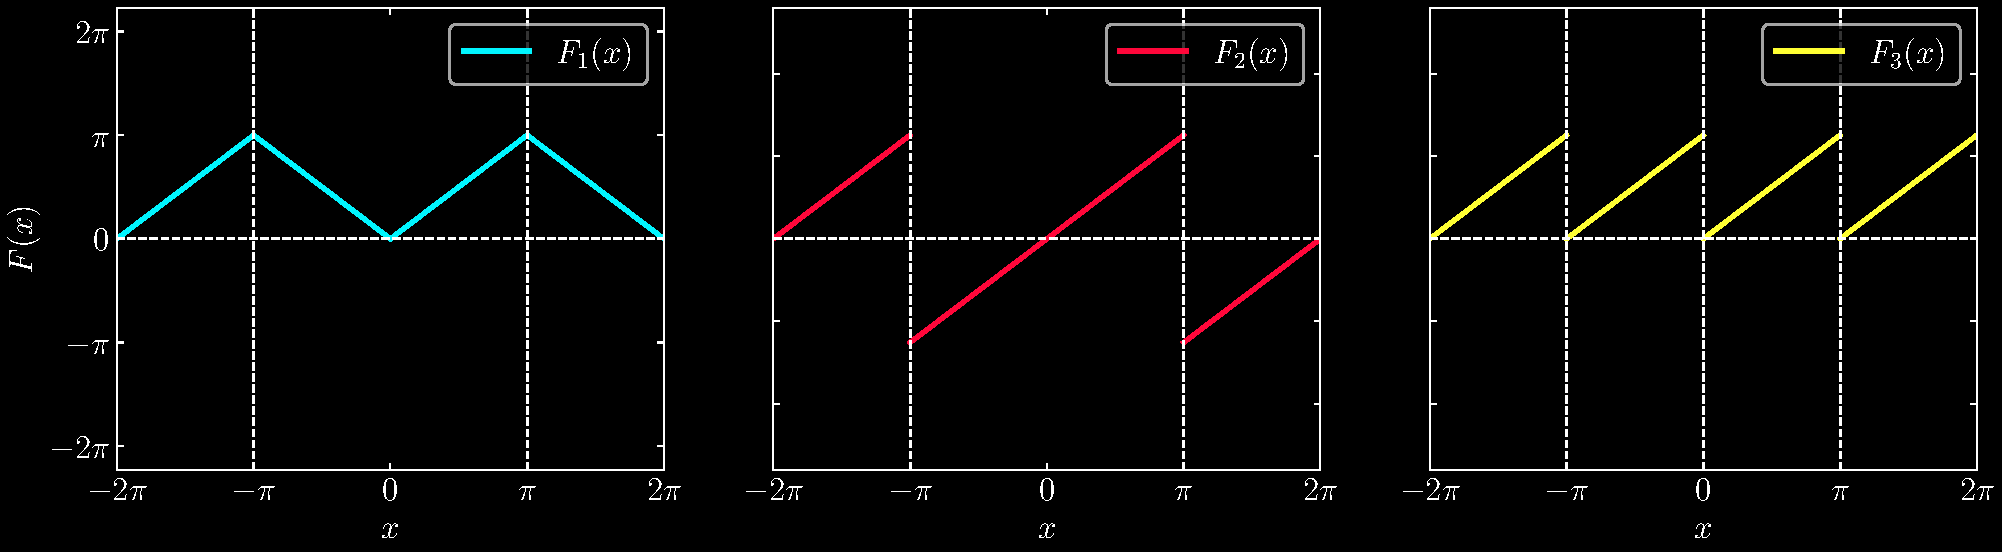
\includegraphics[width=1.0\textwidth]{../chap8/sec8.1/chap8sec8.1ex2.pdf}
\end{center}

% QUESTION 3
\qs{8.1.3}{Find the Fourier series on \( -\pi \le x \le \pi \)  for 
\begin{enumerate}[label=(\alph*)]
	\item \( f_{1}\!\left( x \right) = \sin^{3}\!\left(x\right) \), an odd function (sine series, only two terms)
	\item \( f_{2}\!\left( x \right) = \abs{\sin\!\left(x\right) } \), an even function (cosine series)
	\item \( f_{3}\!\left( x \right) = x \) for \( -\pi \le x \le \pi \) (sine series with jump at \( x = \pi \))
\end{enumerate}}

\begin{enumerate}[label=(\alph*)]
	\item The Fourier coefficients are given by
	\[
		b_{k} = \frac{2}{\pi} \int^{\pi}_{-\pi} \sin^{3}\!\left(x\right) \sin\!\left(kx\right) \, dx  
	\]
	The simplest approach is to write the identity \( \sin\!\left(x\right) = \!\left( e^{ix} - e^{-ix} \right) / 2i \). Then we can calculate
	\begin{align*}
		\sin^{3}\!\left(x\right) & = -\frac{1}{8i} \!\left( e^{ix} - e^{-ix} \right)^{3} \\
	                                 & = -\frac{1}{8i} \!\left( e^{3ix} - e^{-3ix} - 3 \!\left( e^{ix} - e^{-ix} \right) \right) \\ 
					 & = -\frac{1}{4} \!\left( \sin\!\left(3x\right) - 3 \sin\!\left(x\right) \right)
	\end{align*}
	which is a trigonometric identity that itself is also the Fourier series for \( \sin^{3}\!\left(x\right) \), and therefore \( b_{1} = 3/4 \) and \( b_{2} = -1/4 \).
	\item Note that the absolute value means
	\[
		\abs{\sin\!\left(x\right)} = \begin{cases}
			\sin\!\left(x\right) & 0 \le x \le \pi \\
			-\sin\!\left(x\right) & -\pi \le x < 0 \\
		\end{cases} 
	\]
	So calculating \( a_{0} \) yields
	\[
		a_{0} = \frac{1}{2 \pi} \!\left[ \int^{\pi}_{0} \sin\!\left(x\right) \, dx + \int^{0}_{-\pi} \!\left( -\sin\!\left(x\right) \right) \, dx \right] = \frac{2}{\pi}
	\]
	Deriving the Fourier coefficients, we find
	\begin{align*}
		a_{k} & = \frac{2}{\pi} \int^{\pi}_{0} \sin\!\left(x\right) \cos\!\left(kx\right) \, dx \\
		 & = -\frac{1}{\pi} \!\left[ \frac{\cos\!\left(1 - k\right) x}{1 - k} + \frac{\cos\!\left(1 + k\right) x}{1 + k} \right] \Big|^{\pi}_{0} \\
		 & = -\frac{1}{\pi \!\left( k^{2} - 1 \right)} \!\left[ \!\left( 1 + k \right)\cos\!\left(1 - k\right)x + \!\left( 1 - k \right)\cos\!\left(1 + k\right)x \right] \Big|^{\pi}_{0} 
	\end{align*}
	Now, when \( k \) is odd, this expression vanishes. Otherwise, for even \( k \) it reduces to
	\begin{align*}
		 & = \frac{1}{\pi \!\left( k^{2} - 1 \right)} \!\left[ -2 \!\left( 1 + k \right) - 2 \!\left( 1 - k \right) \right] \\
		 & = \frac{4}{\pi \!\left( 1 - k^{2} \right)}
	\end{align*}
	To cleanly put this in a summation, let \( k = 2n \). Then 
	\[
		\abs{\sin\!\left(x\right) } = \frac{2}{\pi} + \frac{4}{\pi} \sum_{n = 1}^{\infty} \frac{\cos\!\left(2nx\right) }{1 - 4n^{2}}, \quad -\pi \le x \le \pi
	\]
	\item The Fourier coefficients are
	\begin{align*}
		b_{k} & = \frac{1}{\pi} \int^{\pi}_{-\pi} x \sin\!\left(kx\right) \, dx \\
		 & = \frac{1}{\pi} \!\left[ \frac{\sin\!\left(kx\right) }{k^{2}} - \frac{x \cos\!\left(kx\right) }{k} \right] \Big|^{\pi}_{-\pi} 
	\end{align*}
	which is \( 2 / k \) when \( k \) is odd and \( -2 / k \) when \( k \) is even. By symmetry, \( b_{0} = 0 \). The Fourier sine series is
	\[
		x = 2 \sum_{n = 1}^{\infty} \frac{\!\left( -1 \right)^{n + 1}}{n} \sin\!\left(nx\right)  
	\]
\end{enumerate}

% QUESTION 4
\qs{8.1.4}{Find the complex Fourier series \( e^{x } = \sum c_{k} e^{ikx} \) on the interval \( -\pi \le x \le \pi \). The even part of a function is \( \frac{1}{2}\!\left( f \!\left( x \right) + f \!\left( -x \right) \right) \), so that \( f_{\text{even}}\!\left( x \right) = f_{\text{even}}\!\left( -x \right) \). Find the cosine series for \( f_{\text{even}} \) and the sine series for \( f_{\text{odd}} \). \textit{Notice the jump at }\( x = \pi \).}

First, we calculate the coefficients to the complex Fourier series as 
\begin{align*}
	c_{k} & = \frac{1}{2 \pi} \int^{\pi}_{-\pi} e^{x} e^{-ikx} \, dx \\
	 & = \frac{1}{2 \pi} \int^{\pi}_{-\pi} e^{\!\left( 1 - ik \right)x} \, dx  \\ 
	 & = \frac{1}{2 \pi} \frac{e^{\!\left( 1 - ik \right)x}}{1 - ik} \Big|^{\pi}_{-\pi} \\
	 & = \frac{1}{2 \pi \!\left( 1 - ik \right)} \!\left[ e^{\!\left( 1 - ik \right)\pi} - e^{-\!\left( 1 - ik \right)\pi} \right]
\end{align*}

Next, decompose the exponential function into the well-known identity
\[
	e^{x} = \underbrace{\frac{1}{2} \!\left( e^{x} + e^{-x} \right)}_{\text{even}} + \underbrace{\frac{1}{2} \!\left( e^{x} - e^{-x} \right)}_{\text{odd}} = \cosh\!\left( x \right) + \sinh\!\left( x \right)
\]

The Fourier cosine series for the even component is

\begin{align*}
	a_{k} & = \int^{\pi}_{-\pi} \frac{1}{2} \!\left( e^{x} + e^{-x} \right) \cos\!\left(kx\right) \, dx \\
	 & = \frac{2}{\pi} \int^{\pi}_{0} \frac{1}{2} \!\left( e^{x} + e^{-x} \right) \cos\!\left(kx\right) \, dx \\ 
	 & = \frac{1}{\pi} \!\left[ \frac{e^{x} \!\left( \cos\!\left(kx\right) + k \sin\!\left(kx\right)  \right)}{1 + k^{2}} + \frac{e^{-x} \!\left( -\cos\!\left(kx\right) + k \sin\!\left(kx\right)  \right)}{1 + k^{2}} \right] \Big|^{\pi}_{0} \\
	 & = \frac{\!\left( -1 \right)^{k}}{\pi} \!\left( \frac{e^{\pi} - e^{-\pi}}{1 + k^{2}} \right) \\
	 & = \!\left( -1 \right)^{k} \frac{2}{\pi \!\left( 1 + k^{2} \right)} \sinh\!\left( \pi \right)
\end{align*}

And for the Fourier sine series for the odd component, we have

\begin{align*}
	b_{k} & = \frac{1}{\pi} \int^{\pi}_{-\pi} \frac{1}{2} \!\left( e^{x} - e^{-x} \right) \sin\!\left(kx\right) \, dx \\
	 & = \frac{2}{\pi} \int^{\pi}_{0} \frac{1}{2} \!\left( e^{x} - e^{-x} \right) \sin\!\left(kx\right) \, dx \\ 
	 & = \frac{1}{\pi} \!\left[ \frac{e^{x} \!\left( \sin\!\left(kx\right) - k \cos\!\left(kx\right) \right)}{1 + k^{2}} - \frac{e^{-x} \!\left( -\sin\!\left(kx\right) - k \cos\!\left(kx\right) \right)}{1 + k^{2}} \right] \Big|^{\pi}_{0} \\
	 & = \!\left( -1 \right)^{k + 1} \frac{k}{\pi} \!\left( \frac{e^{\pi} - e^{-\pi}}{1 + k^{2}} \right) \\
	 & = \!\left( -1 \right)^{k + 1} \frac{2k}{\pi \!\left( 1 + k^{2} \right)} \sinh\!\left(\pi\right) 
\end{align*}

Additionally, the average is
\[
	a_{0} = \frac{1}{2 \pi} \int^{\pi}_{-\pi} e^{x} \, dx = \frac{1}{2 \pi} \!\left( e^{\pi} - e^{-\pi} \right) = \frac{1}{\pi} \sinh\!\left(\pi\right)   
\]
The full Fourier series for our \( F \!\left( x \right) \) is then
\[
	e^{x} = \frac{1}{\pi} \sinh\!\left(\pi\right) + \sum_{k = 1}^{\infty} \!\left( -1 \right)^{k} \frac{2}{\pi \!\left( 1 + k^{2} \right)} \sinh\!\left(\pi\right) \cos\!\left(kx\right) - \sum_{k = 1}^{\infty} \!\left( -1 \right)^{k} \frac{2k}{\pi \!\left( 1 + k^{2} \right)} \sinh\!\left(\pi\right) \sin\!\left(kx\right)  
\]

% QUESTION 5
\qs{8.1.5}{From the energy formula (21), the square wave sine coefficients satisfy
\[
	\pi \!\left( b_{1}^{2} + b_{2}^{2} + \cdots \right) = \int^{\pi}_{-\pi} \abs{SW \!\left( x \right)}^{2} \, dx = \int^{\pi}_{-\pi} 1 \, dx = 2 \pi
\]
Substitute the numbers \( b_{k} \) from equation (8) to find that \( \pi^{2} = 8 \!\left( 1 + \frac{1}{9} + \frac{1}{25} + \cdots \right) \).}	

The coefficients \( b_{k} \) are
\[
	b_{k} = \frac{2}{\pi} \!\left\{ \frac{2}{1}, \frac{2}{3}, \frac{2}{5}, \cdots \right\} 
\]
Substituting gives us
\[
	16 \pi \!\left( \frac{1}{\pi^{2}} + \frac{1}{9 \pi^{2}} + \frac{1}{25 \pi^{2}} + \cdots \right) = 2 \pi \quad \implies \quad \pi^{2} = 8 \!\left( 1 + \frac{1}{9} + \frac{1}{25} + \cdots \right)
\]

% QUESTION 6
\qs{8.1.6}{If a square pulse is centered at \( x = 0 \) to give
\[
	f \!\left( x \right) = 1 \quad \text{for} \quad \abs{x} < \frac{\pi}{2}, \quad f \!\left( x \right) = 0 \quad \text{for} \quad \frac{\pi}{2} < \abs{x} < \pi, 
\]
draw its graph and find its Fourier coefficients \( a_{k} \) and \( b_{k} \).}

\begin{center}
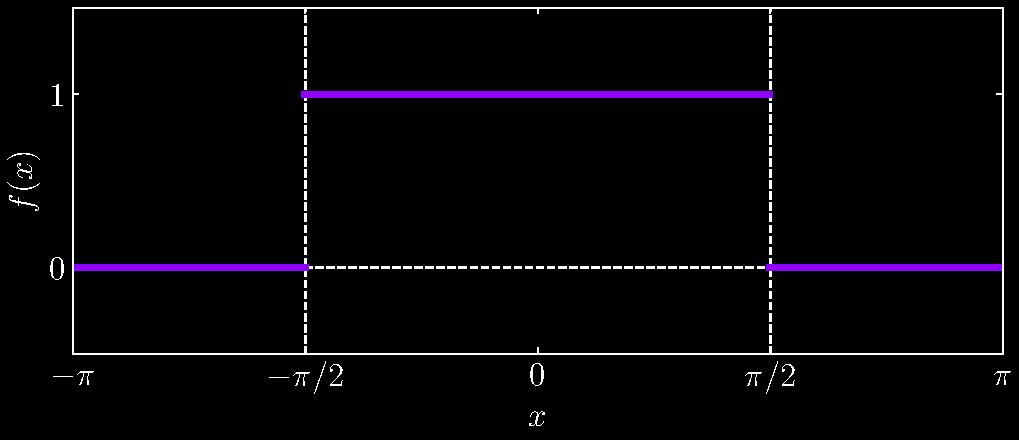
\includegraphics[width=1.0\textwidth]{../chap8/sec8.1/chap8sec8.1ex6.pdf}
\end{center}

On visual inspection, it is apparent that \( f \!\left( x \right) \) is an even function. From that we can immediately conclude that all \( b_{k} = 0 \). Then we calculate
\[
	a_{0} = \frac{1}{2 \pi} \int^{\pi}_{-\pi} f \!\left( x \right) \, dx = \frac{1}{2 \pi} \int^{\pi / 2}_{-\pi / 2}  \, dx = \frac{1}{2} 
\]
\begin{align*}
	a_{k} & = \frac{1}{\pi} \int^{\pi}_{-\pi} f \!\left( x \right) \cos\!\left(kx\right)  \, dx \\
	 & = \frac{1}{\pi} \int^{\pi / 2}_{-\pi / 2} \cos\!\left(kx\right) \, dx \\
	 & = \frac{2}{k \pi} \sin\!\left(\frac{k \pi}{2}\right)
\end{align*}
giving us complete Fourier series
\[
	f \!\left( x \right) = \frac{1}{2} + \sum_{k = 1}^{\infty} \frac{2}{k \pi} \sin\!\left(\frac{k \pi}{2}\right) \cos\!\left(kx\right)  
\]

% QUESTION 7
\qs{8.1.7}{Plot the first three partial sums and the function \( x \!\left( \pi - x \right) \):
\[
	x \!\left( \pi - x \right) = \frac{8}{\pi} \!\left( \frac{\sin\!\left(x\right) }{1} + \frac{\sin\!\left(3x\right) }{27} + \frac{\sin\!\left(5x\right) }{125} + \cdots \right), \quad 0 < x < \pi 
\]
Why is \( 1 / k^{3} \) the decay rate for this function? What is its second derivative?}

\begin{center}
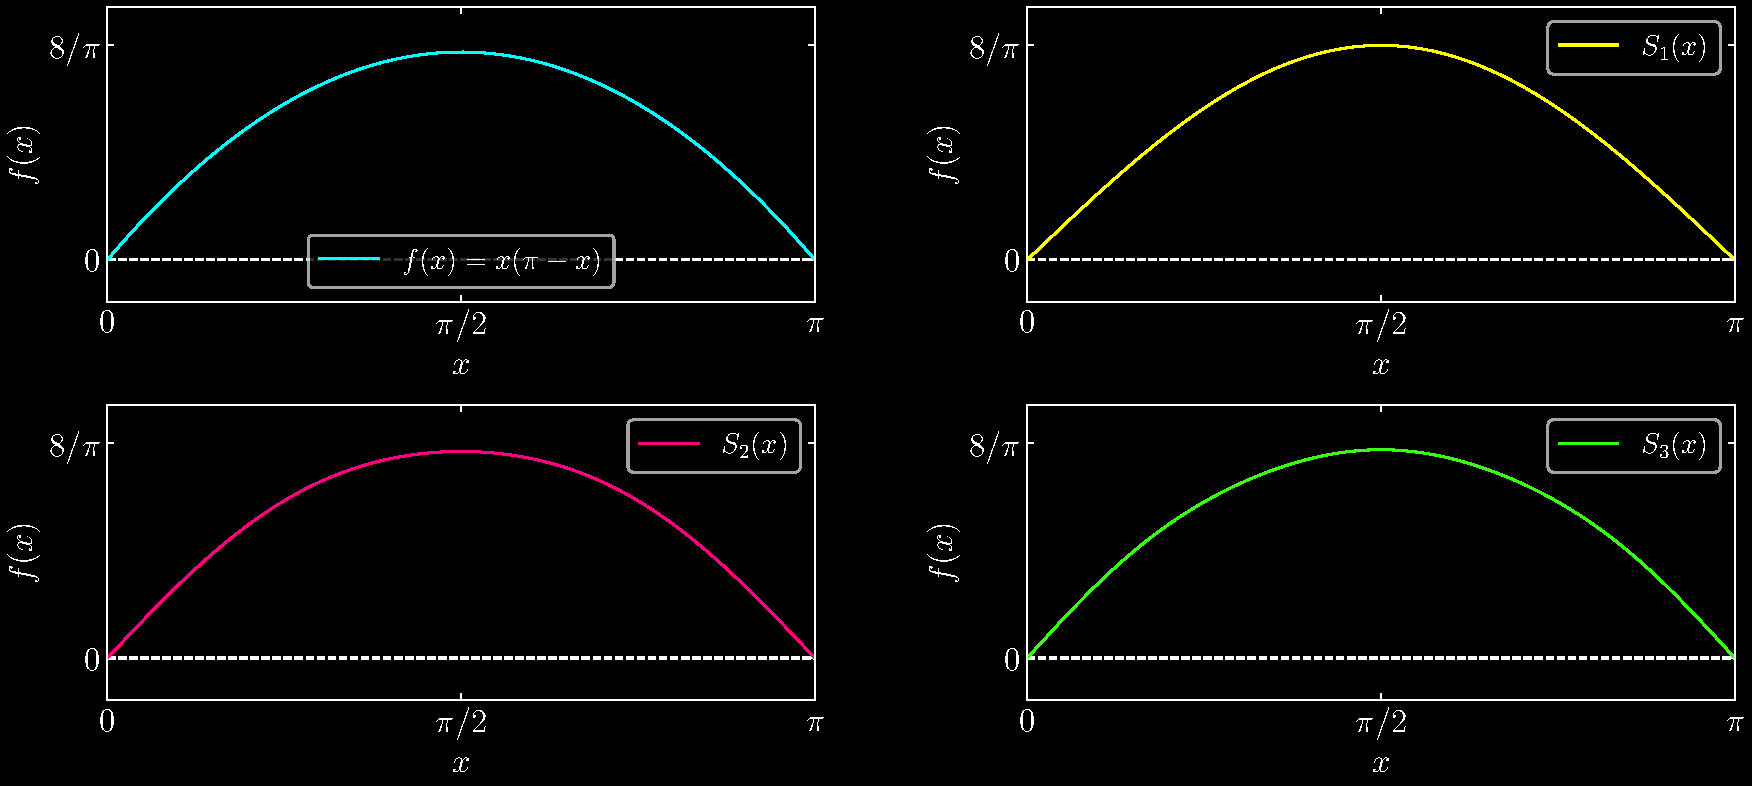
\includegraphics[width=1.0\textwidth]{../chap8/sec8.1/chap8sec8.1ex7.pdf}
\end{center}

The second derivative is \( f'' = -2 \). One analysis here is we must integrate thrice to derive our Fourier coefficient: twice for the \( x^{2} \) term, and once more for the sine. This generates \( 1 / k^{3} \).

Another way to think about the decay rate is as follows: \( 1/k \) corresponds to jumps in the function itself (step functions), \( 1/k^{2} \) is the jump in the first derivative of the ramp function, and \( 1/k^{3} \) for the jump in the second derivative. The argument here, then, requires us to consider the periodic odd extension of \( f \), namely the case where
\[
	f = x \pi + x^{2}, \quad -\pi < x < 0
\]
In this ``branch'', the second derivative is \( +2 \). At \( x = 0 \), we have a discontinuity in the second derivative: the jump from \( +2 \) to \( -2 \).

\vspace{12pt}

% QUESTION 8
\qs{8.1.8}{Sketch the \( 2 \pi \)-periodic half wave with \( f \!\left( x \right) = \sin\!\left(x\right) \) for \( 0 < x < \pi \) and \( f \!\left( x \right) = 0 \) for \( -\pi < x < 0 \). Find its Fourier series.}

\begin{center}
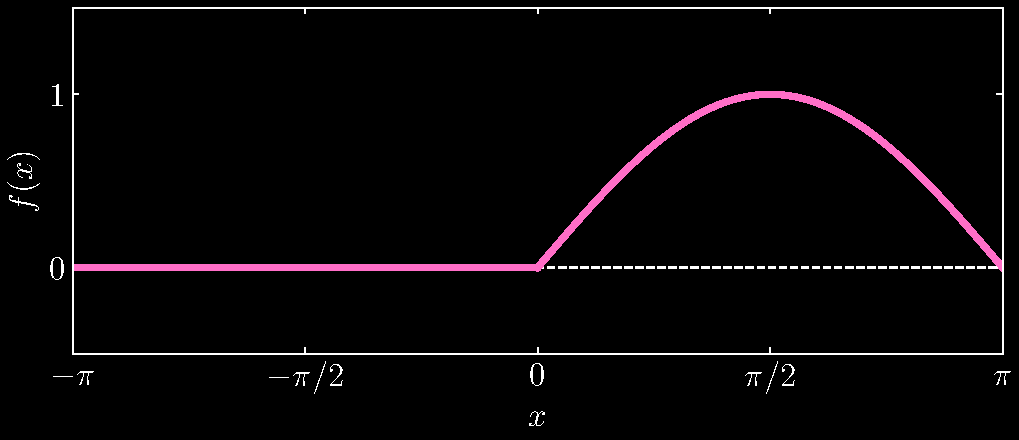
\includegraphics[width=1.0\textwidth]{../chap8/sec8.1/chap8sec8.1ex8.pdf}
\end{center}

The Fourier series is calculated as 
\begin{align*}
	a_{0} & = \frac{1}{2 \pi} \int^{\pi}_{-\pi} f \!\left( x \right) \, dx \\
	 & = \frac{1}{2 \pi} \int^{\pi}_{0} \sin\!\left(x\right) \, dx \\ 
	 & = \frac{1}{\pi} \\
	a_{k} & = \frac{1}{\pi} \int^{\pi}_{0} \sin\!\left(x\right) \cos\!\left(kx\right) \, dx \\
	      & = \frac{1}{\pi} \!\left[ -\frac{\cos\!\left(\!\left( 1 - k \right)x\right) }{2 \!\left( 1 - k \right)} - \frac{\cos\!\left(\!\left( 1 + k \right)x\right) }{2 \!\left( 1 + k \right)} \right] \Big|^{\pi}_{0} \\
	      & = \frac{1}{\pi} \!\left[ \frac{\cos\!\left(k \pi\right) + 1}{2 \!\left( 1 - k \right)} + \frac{\cos\!\left(k \pi\right) + 1}{2 \!\left( 1 + k \right)} \right] \\
\implies a_{n} & = \frac{1}{\pi} \!\left[ \frac{1}{1 - 2n} + \frac{1}{1 + 2n} \right] \quad (\text{substitute } k = 2n \text{; non-zero only for even } k) \\
	      & = \frac{2}{\pi \!\left( 1 - 4n^{2} \right)} \\
	b_{k} & = \frac{1}{\pi} \int^{\pi}_{0} \sin\!\left(x\right) \sin\!\left(kx\right) \, dx \\
	      & = \frac{1}{\pi}\!\left[ \frac{x}{2} - \frac{\sin\!\left(2x\right) }{4} \right] \Big|^{\pi}_{0} \\
	      & = \frac{1}{2}
\end{align*}
which gives us
\[
	f \!\left( x \right) = \frac{1}{\pi} + \sum_{n = 1}^{\infty} \frac{2}{\pi \!\left( 1 - 4n^{2} \right)} + \frac{\sin\!\left(x\right) }{2} 
\]

% QUESTION 9
\qs{8.1.9}{Suppose \( G \!\left( x \right) \) has period \( 2L \) instead of \( 2 \pi \). Then \( G \!\left( x + 2L \right) = G \!\left( x \right) \). Integrals go from \( -L \) to \( L \) or from \( 0 \) to \( 2L \). The Fourier formulas change by a factor \( \pi / L \):

The coefficients in 

\( G \!\left( x \right) = \sum_{-\infty}^{\infty} \pmb{C}_{k} e^{ik \pi x / L} \) are \( \displaystyle{\pmb{C}_{k} = \frac{1}{2L} \int^{L}_{-L} G \!\left( x \right) e^{-ik \pi x / L} \, dx } \).

Derive this formula for \( C_{k} \): Multiply the first equation for \( G \!\left( x \right) \) by \underline{\qquad} and integrate both sides. Why is the integral on the right side equal to \( 2LC_{k} \)?}

Multiply the first equation by \( e^{-ik \pi x / L} \). 
\[
	G \!\left( x \right) e^{-ik \pi x / L} = e^{-ik \pi x / L} \sum_{-\infty}^{\infty} C_{k} e^{ik \pi x / L} 
\]
By orthogonality of the complex exponentials, after integrating, we are left only with 
\[
	\int^{L}_{-L} G \!\left( x \right) e^{-ik \pi x / L} \, dx = \int^{L}_{-L} C_{k} \, dx = 2LC_{k} 
\]

% QUESTION 10
\qs{8.1.10}{For \( G_{\text{even}} \), use Problem 9 to find the cosine coefficient \( A_{k} \) from \( \!\left( C_{k} + C_{-k} \right) / 2 \):
\[
	G_{\text{even}}\!\left( x \right) = \sum_{0}^{\infty} A_{k} \cos\!\left(\frac{k \pi x }{L}\right) \text{ has } A_{k} = \frac{1}{L} \int^{L}_{0} G_{\text{even}}\!\left( x \right) \cos\!\left(\frac{k \pi x}{L}\right) \, dx.  
\]
\( G_{\text{even}} \) is \( \frac{1}{2} \!\left( G \!\left( x \right) + G \!\left( -x \right) \right) \). Exception for \( A_{0} = C_{0} \): Divide by \( 2L \) instead of \( L \).}

Calculate
\begin{align*}
	\frac{c_{k} + c_{-k}}{2} & = \frac{1}{4L} \!\left[ \int^{L}_{-L} G \!\left( x \right) e^{-ik \pi x / L} \, dx + \int^{L}_{-L} G \!\left( x \right) e^{i k \pi x / L} \, dx \right] \\
	 & = \frac{1}{2L} \int^{L}_{-L} G \!\left( x \right) \cos\!\left(\frac{k \pi x }{L}\right) \, dx \\ 
	 & = \frac{1}{2L} \int^{L}_{-L} \!\left[ \underbrace{\frac{1}{2} \!\left( G \!\left( x \right) + G \!\left( -x \right) \right)}_{\text{even}} + \underbrace{\frac{1}{2} \!\left( G \!\left( x \right) - G \!\left( -x \right) \right)}_{\text{odd}} \right] \cos\!\left(\frac{k \pi x }{L}\right) \, dx \\ 
	 & = \frac{1}{2L} \int^{L}_{-L} G_{\text{even}}\!\left( x \right) \cos\!\left(\frac{k \pi x }{L}\right)  \, dx \\
	 & = \frac{1}{L} \int^{L}_{0} G_{\text{even}}\!\left( x \right) \cos\!\left(\frac{k \pi x }{L}\right) \, dx \\
	 & = A_{k}
\end{align*}

Recall that in the third line, since an odd function times an even function is odd, the second integral vanishes over the symmetric bounds. This leaves only the even component of \( G \!\left( x \right) \).

\vspace{12pt}

% QUESTION 11
\qs{8.1.11}{Problem 10 tells us that \( \displaystyle{\pmb{a_{k} = \frac{1}{2} \!\left( c_{k} + c_{-k} \right)}} \) on the usual interval from \( 0 \) to \( \pi \). Find a similar formula for \( b_{k} \) from \( c_{k} \) and \( c_{-k} \). In the reverse direction, find the complex coefficient \( c_{k} \) in \( F \!\left( x \right) = \sum c_{k}e^{ikx} \) from the real coefficients \( a_{k} \) and \( b_{k} \).}

A point of clarification is warranted. Problem 8.1.10 calculates the Fourier coefficient for the \textit{even extension of} \( G \!\left( x \right) \). We can do the same for the \textit{odd} extension of \( G \!\left( x \right) \), which involves reworking the derivation in the previous problem to ensure that the sine term survives. The way to do so is to begin from \( \!\left( c_{k} - c_{-k} \right) / 2 \). Doing so leaves us with
\[
	\frac{c_{k} - c_{-k}}{2} = -\frac{i}{2L} \int^{L}_{-L} G_{\text{odd}}\!\left( x \right)\sin\!\left(\frac{k \pi x }{L}\right) \, dx
\]
Multiply by \( i \) to conclude
\[
	i \!\left( \frac{c_{k} - c_{-k}}{2} \right) = \frac{1}{2L} \int^{L}_{-L} G_{\text{odd}}\!\left( x \right) \sin\!\left(\frac{k \pi x }{L}\right) \, dx = B_{k}
\]
Now, we consider the original function \( G \!\left( x \right) \) (with the definition in Problem 8.1.9). Fix \( k \) and write
\begin{align*}
	c_{k} & = \frac{1}{2L} \int^{L}_{-L} G \!\left( x \right) e^{-ik \pi x / L} \, dx \\
	 & = \frac{1}{2L} \int^{L}_{-L} G \!\left( x \right) \!\left[ \cos\!\left(\frac{k \pi x}{L}\right) - i \sin\!\left(\frac{k \pi x}{L}\right) \right] \, dx \\ 
	 & = \frac{1}{2} \!\left( a_{k} - i b_{k} \right)
\end{align*}
Analogously conclude that
\[
	c_{-k} = \frac{1}{2} \!\left( a_{k} + i b_{k} \right) 
\]
Two equations for two unknowns gives us
\begin{align*}
	a_{k} & = c_{k} + c_{-k} \\
	b_{k} & = i \!\left( c_{k} - c_{-k} \right)
\end{align*}
which are the great and elegant formulae for relating the complex and trigonometric Fourier coefficients for \( G \!\left( x \right) \).

\vspace{12pt}

% QUESTION 12
\qs{8.1.12}{Find the solution to Laplace's equation with \( u_{0} = \theta \) on the boundary. Why is this the imaginary part of \( 2 \!\left( z - z^{2} / 2 + z^{3} / 3 \cdots \right) = 2 \log\!\left( 1 + z \right) \)? Confirm that on the unit circle \( z = e^{i \theta} \), the imaginary part of \( 2 \log\!\left( 1 + z \right) \) agrees with \( \theta \).}

Since \( u_{0} \!\left( \theta \right) = \theta \) is an odd function, we calculate the sine series as 
\begin{align*}
	b_{0} & = \frac{1}{\pi} \int^{\pi}_{-\pi} \theta \, d \theta \\
	 & = 0 \\ 
	b_{k} & = \frac{1}{\pi} \int^{\pi}_{-\pi} \theta \sin\!\left(k \theta\right) \, d \theta \\
	      & = \frac{1}{\pi} \!\left[ \frac{\sin\!\left(k \theta\right)}{k^{2}} - \frac{\theta \cos\!\left(k \theta\right)}{k} \right] \Big|^{\pi}_{-\pi} \\
	      & = \frac{2}{k}\!\left( -1 \right)^{k + 1}
\end{align*}

The solution to Laplace's equation is
\[
	u\!\left( r, \theta \right) = \frac{2}{1}r \sin\!\left(\theta\right) - \frac{2}{2}r^{2}\sin\!\left(2 \theta\right) + \frac{2}{3}r^{3}\sin\!\left(3 \theta\right) - \cdots = \sum_{k = 1}^{\infty} \frac{2}{k}\!\left( -1 \right)^{k + 1}r^{k} \sin\!\left(k \theta\right)  
\]
Let \( z = re^{i \theta} \). Then this solution indeed corresponds to \( \Imag \!\left[ 2 \log \!\left( 1 + z \right) \right] \).

\vspace{12pt}

% QUESTION 13
\qs{8.1.13}{If the boundary condition for Laplace's equation is \( u_{0} = 1 \) for \( 0 < \theta < \pi \) and \( u_{0} = 0 \) for \( -\pi < \theta < 0 \), find the Fourier series solution \( u \!\left( r, \theta \right) \) inside the unit circle. What is \( u \) at the origin \( r = 0 \)?}

We must calculate the complete Fourier series, which is
\begin{align*}
	a_{0} & = \frac{1}{2 \pi} \int^{\pi}_{-\pi} u_{0} \, d \theta \\
	 & = \frac{1}{2 \pi} \int^{\pi}_{0} \, d \theta \\ 
	 & = \frac{1}{2} \\
	a_{k} & = \frac{1}{\pi} \int^{\pi}_{0} \cos\!\left(k \theta\right) \, d \theta \\
	      & = 0 \\
	b_{k} & = \frac{1}{\pi} \int^{\pi}_{0} \sin\!\left(k \theta\right) \, d \theta \\
	      & = \frac{1}{\pi} \!\left[ \frac{\!\left( -1 \right)^{k + 1} + 1}{k} \right]
\end{align*}
This vanishes for even \( k \), so we should write
\[
	b_{n} = \frac{2}{\pi \!\left( 2n - 1 \right)} 
\]
The solution to Laplace's equation is
\[
	u \!\left( r, \theta \right) = \frac{1}{2} + \sum_{n = 1}^{\infty} \frac{2}{\pi \!\left( 2n - 1 \right)} r^{2n - 1} \sin\!\left(\!\left( 2n - 1 \right) \theta \right)
\]

% QUESTION 14
\qs{8.1.14}{With boundary values \( u_{0}\!\left( \theta \right) = 1 + \frac{1}{2}e^{i \theta} + \frac{1}{4}e^{2i \theta} + \cdots \), what is the Fourier series solution to Laplace's equation in the circle? Sum this geometric series.}

Multiply each term by the corresponding power of \( r \) to get
\[
	u \!\left( r, \theta \right) = \sum_{n = 0}^{\infty} \!\left( \frac{1}{2}re^{i \theta} \right)^{n}
\]
For this infinite sum, we have closed-form expression
\[
	u \!\left( r, \theta \right) = \frac{1}{1 - \frac{1}{2}re^{i \theta}}
\]

% QUESTION 15
\qs{8.1.15}{
\begin{enumerate}[label=(\alph*)]
	\item Verify that the fraction in Poisson's formula (30) satisfies Laplace's equation.
	\item Find the response \( u \!\left( r, \theta \right) \) to an impulse at \( x = 0 \), \( y = 1 \) (where \( \theta = \frac{\pi}{2} \)).
\end{enumerate}}

\begin{enumerate}[label=(\alph*)]
	\item In \( \!\left( r, \theta \right) \) coordinates, Laplace's equation is
	\[
		\frac{\partial^{2} u}{\partial r^{2}} + \frac{1}{r} \frac{\partial u}{\partial r} + \frac{1}{r^{2}} \frac{\partial^{2} u}{\partial \theta^{2}} = 0
	\]
	Note that the Poisson's equation has, for the purposes of differentiation, a more legible summation form
	\[
		u \!\left( r, \theta \right) = \frac{1}{2 \pi} + \frac{1}{\pi} \sum_{n = 1}^{\infty} r^{n}\cos\!\left(n \theta\right) 
	\]
	Each term is calculated as 
	\begin{align*}
		\frac{\partial^{2} u}{\partial r^{2}} & = \frac{1}{\pi} \sum_{n = 1}^{\infty} n \!\left( n - 1 \right) r^{n - 2} \cos\!\left(n \theta\right) \\
		\frac{1}{r} \frac{\partial u}{\partial r} & = \frac{1}{\pi} \sum_{n = 1}^{\infty} nr^{n - 2} \cos\!\left(n \theta\right) \\
		\frac{1}{r^{2}} \frac{\partial^{2} u}{\partial \theta^{2}} & = -\frac{1}{\pi} \sum_{n = 1}^{\infty} n^{2}r^{n - 2} \cos\!\left(n \theta\right) 
	\end{align*}
	which, expectedly, vanish upon summation.
	\item Think of the impulse as undergoing an angular displacement of \( \theta = \pi / 2 \). The phase shift \( \cos\!\left(\theta + \pi / 2 \right) \) becomes \( -\sin\!\left(\theta\right) \). Poisson's equation becomes
	\[
		u \!\left( r, \theta \right) = \frac{1}{2 \pi} \frac{1 - r^{2}}{1 + r^{2} + 2r \sin\!\left(\theta\right) } 
	\]
\end{enumerate}

% QUESTION 16
\qs{8.1.16}{With complex exponentials in \( F \!\left( x \right) = \sum c_{k}e^{ikx} \), the energy identity (21) changes to \( \int^{\pi}_{-\pi} \abs{F \!\left( x \right)}^{2} \, dx = 2 \pi \sum \abs{c_{k}}^{2} \). Derive this by integrating \( \!\left( \sum c_{k}e^{ikx} \right)\!\left( \sum \overline{c}_{k}e^{-ikx} \right) \).}

By orthogonality, we know that surviving terms will only be those with the same \( k \) in both summations. This leaves us with
\[
	\int^{\pi}_{-\pi} \sum \abs{c_{k}}^{2} \, dx = 2 \pi \sum \abs{c_{k}}^{2} 
\]

% QUESTION 17
\qs{8.1.17}{A centered square wave has \( F \!\left( x \right) = 1 \) for \( \abs{x} \le \pi / 2 \).
\begin{enumerate}[label=(\alph*)]
	\item Find its energy \( \int \abs{F \!\left( x \right)}^{2} \, dx \) by direct integration
	\item Compute its Fourier coefficients \( c_{k} \) as specific numbers
	\item Find the sum in the energy identity (Problem 16).
\end{enumerate}}

\begin{enumerate}[label=(\alph*)]
	\item 
	\[
		\int^{\pi}_{-\pi} \abs{F \!\left( x \right)}^{2} \, dx = \int^{\pi / 2}_{-\pi / 2} \, dx = \pi   
	\]
	\item 
	\begin{align*}
		c_{k} & = \frac{1}{2 \pi} \int^{\pi / 2}_{-\pi / 2} e^{-ikx} \, dx \\ 
		      & = -\frac{1}{2 \pi ik} \!\left( e^{-ik \pi / 2} - e^{i k \pi / 2} \right) \\ 
		      & = \frac{1}{\pi k} \sin\!\left(\frac{k \pi}{2}\right)
	\end{align*}
	In general, the squared coefficients take on form
	\[
		\abs{c_{k}}^{2} = 
		\begin{cases}
			\displaystyle{\frac{1}{4}}, & k = 0 \\
			\displaystyle{\frac{1}{\pi^{2} \!\left( 2k - 1 \right)^{2}}}, & k > 0
		\end{cases}
	\]
	\item 
	Since we need to sum over all integers (positive, negative, and zero), we need to multiply the summation here by two to account for the negatives (as it only sums from \( k = 1 \) onward), and add \( \abs{c_{0}^{2}} \).
	\begin{align*}
		\int^{\pi}_{-\pi} \sum \abs{c_{k}}^{2} \, dx & = 2 \pi \sum_{-\infty}^{\infty}  \abs{c_{k}}^{2} \\
										& = 2 \pi \!\left( \abs{c_{0}}^{2} + \sum_{k = 1}^{\infty} \!\left( \abs{c_{k}}^{2} + \abs{c_{-k}}^{2} \right) \right) \\
										& = 2 \pi \!\left( \abs{c_{0}}^{2} + 2 \sum_{k = 1}^{\infty} \abs{c_{k}}^{2} \right) \\
		 & = 2 \pi \!\left( \frac{1}{4} + 2 \sum \frac{1}{\pi^{2} \!\left( 2k - 1 \right)^{2}} \right) \\ 
		 & = 2 \pi \!\left( \frac{1}{4} + \frac{1}{4} \right) \\
		 & = \pi
	\end{align*}
\end{enumerate}

% QUESTION 18
\qs{8.1.18}{\( F \!\left( x \right) = 1 + \!\left( \cos\!\left(x\right) \right) / 2 + \cdots + \!\left( \cos\!\left(nx\right) \right) / 2^{n} + \cdots \) is analytic: infinitely smooth.
\begin{enumerate}[label=(\alph*)]
	\item If you take 10 derivatives, what is the Fourier series of \( d^{10} F / dx^{10} \)?
	\item Does that series still converge quickly? Compare \( n^{10} \) with \( 2^{n} \) for \( n = 2^{10} \).
\end{enumerate}}

\begin{enumerate}[label=(\alph*)]
	\item We have
	\[
		F^{10}\!\left( x \right) = - \!\left[ \frac{\cos\!\left(x\right) }{2} + \cdots + \frac{n^{10}\cos\!\left(nx\right) }{2^{n}} + \cdots \right] = -\sum_{k = 1}^{\infty} \frac{k^{10}\cos\!\left(kx\right) }{2^{k}}
	\]
	which is indeed its own Fourier series.
	\item Yes; \( \!\left( 2^{10} \right)^{10} = 2^{100} \) is immensely less than \( 2^{2^{10}} \). In general, \( n^{10} \) grows much slower than \( 2^{n} \) for large \( n \).
\end{enumerate}

% QUESTION 19
\qs{8.1.19}{If \( f \!\left( x \right) = 1 \) for \( \abs{x} \le \pi / 2\) and \( f \!\left( x \right) = 0 \) for \( \pi / 2 < \abs{x} < \pi \), find its cosine coefficients. Can you graph and compute the Gibbs overshoot at the jumps?}

The cosine coefficients are
\[
	a_{k} = \frac{1}{\pi} \int^{\pi / 2}_{-\pi / 2} \cos\!\left(kx\right) \, dx = \frac{2}{\pi k} \sin\!\left(\frac{k \pi}{2}\right)
\]
which reduces to
\[
	a_{n} = \!\left( -1 \right)^{n + 1}\frac{2}{\pi \!\left( 2n - 1 \right)}
\]
Since \( a_{0} = 1/2 \), the Fourier cosine series is
\[
	f \!\left( x \right) = \frac{1}{2} + \sum_{n = 1}^{\infty} \!\left( -1 \right)^{n + 1}\frac{2}{\pi \!\left( 2n - 1 \right)} \cos\!\left(\!\left( 2n - 1 \right)x\right) 
\]

The Gibbs overshoot for numerous values of partial sums \( S_{N} \) is
\begin{center}
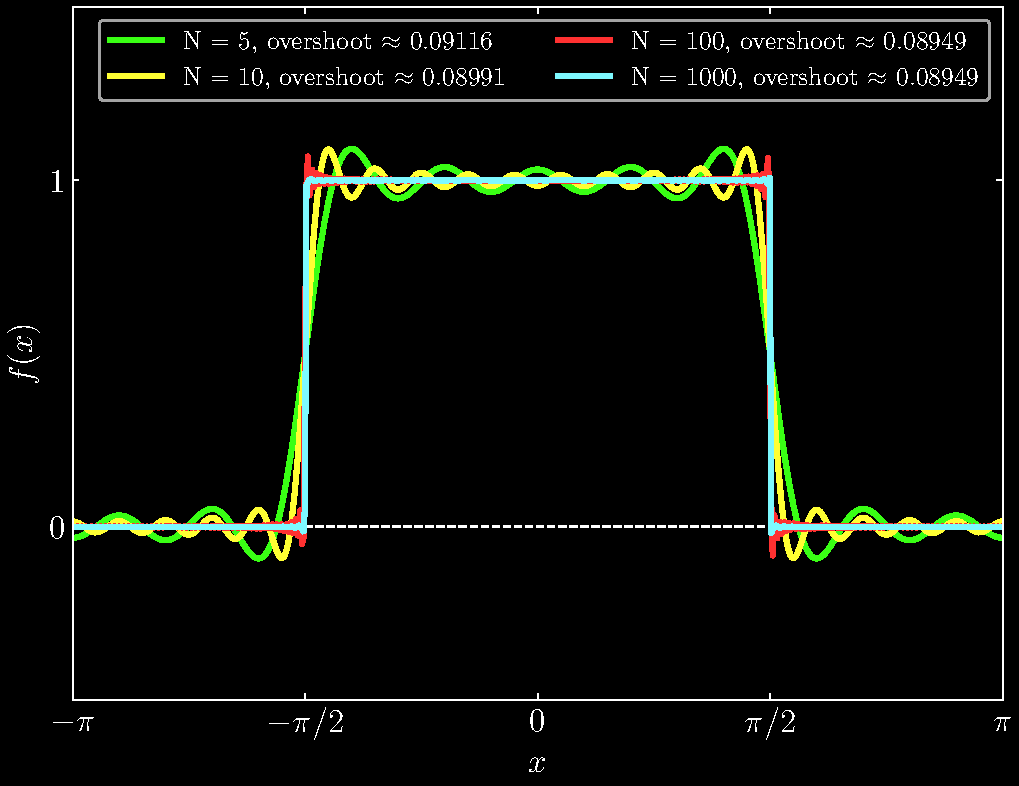
\includegraphics[width=1.0\textwidth]{../chap8/sec8.1/chap8sec8.1ex19.pdf}
\end{center}

\newpage
% QUESTION 20
\qs{8.1.20}{Find all the coefficients \( a_{k} \) and \( b_{k} \) for \( F \), \( I \), and \( D \) on the interval \( -\pi \le x \le \pi \):
\[
	F \!\left( x \right) = \delta \!\left( x - \frac{\pi}{2} \right) \quad I \!\left( x \right) = \int^{x}_{0} \delta \!\left( x - \frac{\pi}{2} \right) \, dx \quad D \!\left( x \right) = \frac{d }{d x} \delta \!\left( x - \frac{\pi}{2} \right)  
\]}

\( F \!\left( x \right) \):

\begin{align*}
	a_{0} & = \frac{1}{2 \pi} \int^{\pi}_{-\pi} \delta\!\left( x - \frac{\pi}{2} \right) \, dx \\ 
	a_{k} & = \frac{1}{\pi} \int^{\pi}_{-\pi} \cos\!\left(kx\right) \delta\!\left( x - \frac{\pi}{2} \right) \, dx \\
	 & = \frac{1}{\pi} \cos\!\left(\frac{k \pi}{2}\right) \\
	b_{k} & = \frac{1}{\pi} \int^{\pi}_{-\pi} \sin\!\left(kx\right) \delta\!\left( x - \frac{\pi}{2} \right) \, dx \\
	      & = \frac{1}{\pi} \sin\!\left(\frac{k \pi}{2}\right) 
\end{align*}

\( I \!\left( x \right) \): Note that this \( I \!\left( x \right) \) is a definition of the Heaviside step function \( \displaystyle{H \!\left( x - \frac{\pi}{2} \right)} \).

\begin{align*}
	a_{0} & = \frac{1}{2 \pi} \int^{\pi}_{-\pi} \int^{x}_{0} \delta\!\left( x - \frac{\pi}{2} \right) \, dx \, dx \\
	 & = \frac{1}{2 \pi} \int^{\pi}_{-\pi} H \!\left( x - \frac{\pi}{2} \right) \, dx \\ 
	 & = \frac{1}{4} \\
	a_{k} & = \frac{1}{\pi} \int^{\pi}_{-\pi} \cos\!\left(kx\right) H \!\left( x - \frac{\pi}{2} \right) \, dx \\
	      & = \frac{1}{\pi k} \!\left[ \sin\!\left(k \pi\right) - \sin\!\left(\frac{k \pi}{2}\right) \right] \\
	      & = -\frac{1}{\pi k} \sin\!\left(\frac{k \pi}{2}\right) \\
	b_{k} & = \frac{1}{\pi} \int^{\pi}_{-\pi} \sin\!\left(kx\right) H \!\left( x - \frac{\pi}{2} \right) \, dx \\
	      & = \frac{1}{\pi k} \!\left[ \cos\!\left(\frac{k \pi}{2}\right) - \cos\!\left(k \pi\right) \right]
\end{align*}

\( D \!\left( x \right) \): Relying on the intuition of integration by parts is key, although remember that the delta function is not a ``function'' in the rigorous sense (for reasons beyond our scope here).

For \( a_{0} \), let \( u = 1 \) and \( dv = \displaystyle{\frac{d }{d x} \delta\!\left( x - \frac{\pi}{2} \right)} \, dx \). Then \( du = 0 \) and \( v = \displaystyle{\delta\!\left( x - \frac{\pi}{2} \right)} \).
\begin{align*}
	a_{0} & = \frac{1}{2 \pi} \int^{\pi}_{-\pi} \frac{d }{d x} \delta \!\left( x - \frac{\pi}{2} \right) \, dx \\
	      & = \frac{1}{2 \pi} \delta \!\left( x - \frac{\pi}{2} \right) \Big|^{\pi}_{-\pi} \\ 
	      & = 0
\end{align*}
In the cases of \( a_{k} \) and \( b_{k} \), let \( u = \cos\!\left(kx\right) \) or \( u = \sin\!\left(kx\right) \), corresponding to \( du = -k \sin\!\left(kx\right) \) or \( du = k \cos\!\left(kx\right) \).
\begin{align*}
	a_{k} & = \frac{1}{2 \pi} \int^{\pi}_{-\pi} \cos\!\left(kx\right) \frac{d }{d x} \delta\!\left( x - \frac{\pi}{2} \right) \, dx \\
	 & = -\frac{k}{2 \pi} \int^{\pi}_{-\pi} \sin\!\left(kx\right) \delta\!\left( x - \frac{\pi}{2} \right) \, dx \\
	 & = -\frac{k}{2 \pi} \sin\!\left(\frac{k \pi}{2}\right) \\
	b_{k} & = \frac{1}{2 \pi} \int^{\pi}_{-\pi} \sin\!\left(kx\right) \frac{d }{d x} \delta\!\left( x - \frac{\pi}{2} \right) \, dx \\
	      & = \frac{k}{2 \pi} \int^{\pi}_{-\pi} \cos\!\left(kx\right) \delta\!\left( x - \frac{\pi}{2} \right) \, dx \\
	      & = \frac{k}{2 \pi} \cos\!\left(kx\right) 
\end{align*}
Observe that \( a_{k} \) and \( b_{k} \) here are the Fourier coefficients of the step functioncase multipled by \( k \).

\vspace{12pt}

% QUESTION 21
\qs{8.1.21}{For the one-sided tall box function in Example 4, with \( F = 1/h \) for \( 0 \le x \le h \), what is its odd part \( \frac{1}{2}\!\left( F \!\left( x \right) - F \!\left( -x \right) \right) \)? I am surprised that the Fourier coefficients of this odd part disappear as \( h \) approaches zero and \( F \!\left( x \right) \) approaches \( \delta\!\left( x \right) \).}

In order for the even and odd decomposition to work, we should clarify that our \( F \) is defined over a symmetric interval \( -h \le x \le h \), namely
\[
	F \!\left( x \right) = 
	\begin{cases}
		1 / h, & 0 \le x \le h \\
		0, & -h \le x < 0 \\
	\end{cases}
\]
Given the piecewise nature of this function, we must calculate the odd part on each interval. First, over \( 0 \le x \le h \):
\[
	F_{\text{odd}} = \frac{1}{2}\!\left( \frac{1}{h} - 0 \right) = \frac{1}{2h}
\]
and secondly, over \( -h \le x < 0 \):
\[
	F_{\text{odd}} = \frac{1}{2}\!\left( 0 - \frac{1}{h} \right) = -\frac{1}{2h} 
\]
Now we calculate the Fourier coefficients
\begin{align*}
	a_{0} & = \frac{1}{2 h} \int^{h}_{-h} F \!\left( x \right) \, dx \\
	 & = \frac{1}{2 h} \!\left[ \int^{h}_{0} \frac{1}{2h} \, dx - \int^{0}_{-h} \frac{1}{2h} \, dx \right] \\ 
	 & = \frac{1}{2 h} \!\left[ \frac{1}{2} - \frac{1}{2} \right] \\
	 & = 0 \\
	a_{k} & = \frac{1}{h} \int^{h}_{-h} F \!\left( x \right) \cos\!\left(kx\right) \, dx  \\
	 & = \frac{1}{2h^{2}} \!\left[ \int^{h}_{0} \cos\!\left(kx\right) \, dx - \int^{0}_{-h} \cos\!\left(kx\right) \, dx \right] \\
	 & = 0 \\
	b_{k} & = \frac{1}{\pi} \int^{h}_{-h} F \!\left( x \right)\sin\!\left(kx\right) \, dx \\
	 & = \frac{1}{2 \pi h} \!\left[ \int^{h}_{0} \sin\!\left(kx\right) \, dx - \int^{0}_{-h} \sin\!\left(kx\right) \, dx \right] \\
	 & = \frac{1}{2 \pi kh} \!\left[ -\cos\!\left(kh\right) + 1 + 1 - \cos\!\left(kh\right) \right] \\
	 & = \frac{\cos\!\left(kh\right) - 1}{\pi k h}
\end{align*}

In the limit, we can apply l'H\^{o}pital's rule to find that \( b_{k} \rightarrow 0 \) as \( h \rightarrow 0 \), though \( b_{k} \) is never truly zero.

\vspace{12pt}

% QUESTION 22
\qs{8.1.22}{Find the series \( F \!\left( x \right) = \sum c_{k}e^{ikx} \) for \( F \!\left( x \right) = e^{x} \) on \( -\pi \le x \le \pi \). That function \( e^{x} \) looks smooth, but there must be a hidden jump to get coefficients \( c_{k} \) proportional to \( 1 / k \). Where is the jump?}

The coefficients are
\begin{align*}
	c_{k} & = \frac{1}{2 \pi} \int^{\pi}_{-\pi} e^{x}e^{-ikx} \, dx \\
	 & = \frac{1}{2 \pi} \int^{\pi}_{-\pi} e^{\!\left( 1 - ik \right)x} \, dx \\
	 & = \frac{1}{2 \pi \!\left( 1 - ik \right)} e^{\!\left( 1 - ik \right)x} \Big|^{\pi}_{-\pi} \\
	 & = \frac{1}{2 \pi \!\left( 1 - ik \right)} \!\left[ e^{\!\left( 1 - ik \right)\pi } - e^{-\!\left( 1 - ik \right) \pi} \right] \\
	 & = \frac{\!\left( -1 \right)^{k}}{2 \pi \!\left( 1 - ik \right)} \!\left[ e^{\pi} - e^{-\pi} \right]
\end{align*}

The jumps occur at every \( x = \!\left( 2k + 1 \right)\pi \), where we go from \( e^{\pi} \) down to \( e^{-\pi} \). That jump appears as a factor in the Fourier coefficients.

\vspace{12pt}

% QUESTION 23
\qs{8.1.23}{\begin{enumerate}[label=(\alph*)]
	\item (Old particular solution) Solve \( Ay'' + By' + Cy = e^{ikx} \).
	\item (New particular solution) Solve \( Ay'' + By' + Cy = \sum c_{k}e^{ikx} \).
\end{enumerate}}

\begin{enumerate}[label=(\alph*)]
	\item Let \( y_{p} = Y_{k}e^{ikx} \). Then \( y'' = -k^{2}Y_{k}e^{ikx} \) and \( y' = ikY_{k}e^{ikx} \). We have
	\[
		-k^{2}Y_{k}A + ikY_{k}B + Y_{k}C = 1 \quad \implies \quad Y_{k} = \frac{1}{C - k^{2}A + ikB}
	\]
	\item By superposition,
	\[
		y_{p} = \sum c_{k}Y_{k}e^{ikx}
	\]
\end{enumerate}

\end{document}
